%
% Szakdolgozatminta az Eszterházy Károly Katolikus Egyetem
% matematika illetve informatika szakos hallgatóinak.
%

\documentclass[
% opciók nélkül: egyoldalas nyomtatás, elektronikus verzió
% twoside,     % kétoldalas nyomtatás
% tocnopagenum,% oldalszámozás a tartalomjegyzék után kezdődik
]{thesis-ekf}
\usepackage[T1]{fontenc}
\PassOptionsToPackage{defaults=hu-min}{magyar.ldf}
\usepackage[magyar]{babel}
\usepackage{mathtools,amssymb,amsthm,pdfpages}
\footnotestyle{rule=fourth}

\newtheorem{tetel}{Tétel}[chapter]
\theoremstyle{definition}
\newtheorem{definicio}[tetel]{Definíció}
\theoremstyle{remark}
\newtheorem{megjegyzes}[tetel]{Megjegyzés}

\begin{document}
\institute{Matematikai és Informatikai Intézet}
\title{Határidő napló webes és androidos platformon}
\author{Kertész Zoltán\\Programtervező informatikus BSc}
\supervisor{Dr. Tajti Tibor Gábor\\adjuntus}
\city{Eger}
\date{2022}
\maketitle
\tableofcontents

\chapter*{Bevezetés}
\addcontentsline{toc}{chapter}{Bevezetés}
A tanulmányaim alatt lehetőségem volt többféle programozási nyelv megismerésére. A szerver és a kliens oldali programozási nyelvek között is találtam olyat, ami elnyerte a tetszésemet. 

A mobil applikáció fejlesztéssel először egy beadandó feladatban találkoztam, majd később az ehhez tartozó órákat is elvégeztem, hogy elmélyítsem a tudásomat. A Java programozási nyelv elsajátítása nem okozott nagy kihívást köszönhetően a tanáraimnak. 

A weboldal fejlesztési ismeretek úgy gondolom, hogy manapság egy alapvető elvárás ezért több erre szolgáló programozási nyelvet is tanultam, de ezek közül az PHP volt számomra a legkedveltebb. A választék igen nagy a PHP alapú keretrendszerek között, de számomra a Laravel lett a preferált.

Ezért az lett a célom, hogy szakdolgozatomban ezeket a technológiákat használjam. Ezek felhasználásra rengeteg terv volt a fejemben, mire kialakult a jelenlegi projekt.

Véleményem szerint az emberek manapság inkább különböző applikációkat használnak, hogy a teendőiket nyilvántartsák, mint a hagyományos papír alapú noteszt. Viszont csak a mobilon tárolni a fontos feljegyzéseinket veszélyes, mivel az egy sérülékeny eszköz. A dolgozatom lényege, hogy egy olyan alkalmazást hozzak létre, amiben a felhasználók el tudják tárolni az eseményeiket és el is érjék azokat távolról is, platform függetlenül. Mivel az okos telefonok rendelkeznek beépített böngészővel így elég lenne, a probléma megoldásához csak a webes alkalmazás is, de szívesebben használják a felhasználók a kliens programokat. 

\chapter{Az alkalmazás}
A szakdolgozatom projektje két részből tevődik össze. Az első rész egy webes alkalmazás a második pedig egy mobil applikáció. A fő összetevője a webes felület, mivel Androidon a projekt nem minden funkciója érhető el. 

A web alkalmazásban törekedtem egy minimalista, mégis modern dizájn kialakításra
\section{Webes alkalmazás}

\section{Androidos alkalmazás}


\begin{tetel}
Tétel szövege.
\end{tetel}

\begin{proof}
Bizonyítás szövege.
\end{proof}

\begin{definicio}
Definíció szövege.
\end{definicio}

\begin{megjegyzes}
Megjegyzés szövege.
\end{megjegyzes}

\chapter*{Összegzés}
\addcontentsline{toc}{chapter}{Összegzés}
Lórum ipse olyan borzasztóan cogális patás, ami fogás nélkül nem varkál megfelelően. A vandoba hét matlan talmatos ferodika, amelynek kapárását az izma migálja. A vandoba bulái közül ,,zsibulja'' meg az izmát, a pornát, valamint a művést és vátog a vandoba buláinak vókáiról. Vókája a raktil prozása két emen között. Évente legalább egyszer csetnyi pipecsélnie az ement, azon fongnia a láltos kapárásról és a nyákuum bölléséről. A vandoba ninti és az emen elé redőzi a szamlan radalmakan érvést. Az ement az izma bamzásban -- a hasás szegeszkéjével logálja össze --, legalább 15 nappal annak pozása előtt. Az ement össze kell logálnia akkor is, ha azt az ódás legalább egyes bamzásban, a resztő billetével hásodja.

\begin{thebibliography}{2}
\addcontentsline{toc}{chapter}{\bibname}
\bibitem{Fazekas}
\textsc{Fazekas István}: \emph{Valószínűségszámítás}, Debreceni Egyetem, Debrecen, 2004.
\bibitem{Tomacs}
\textsc{Tómács Tibor}: \emph{A valószínűségszámítás alapjai}, Líceum Kiadó, Eger, 2005.
\end{thebibliography}

% Aláírt, szkennelt nyilatkozat beillesztése a szakdolgozat végére
%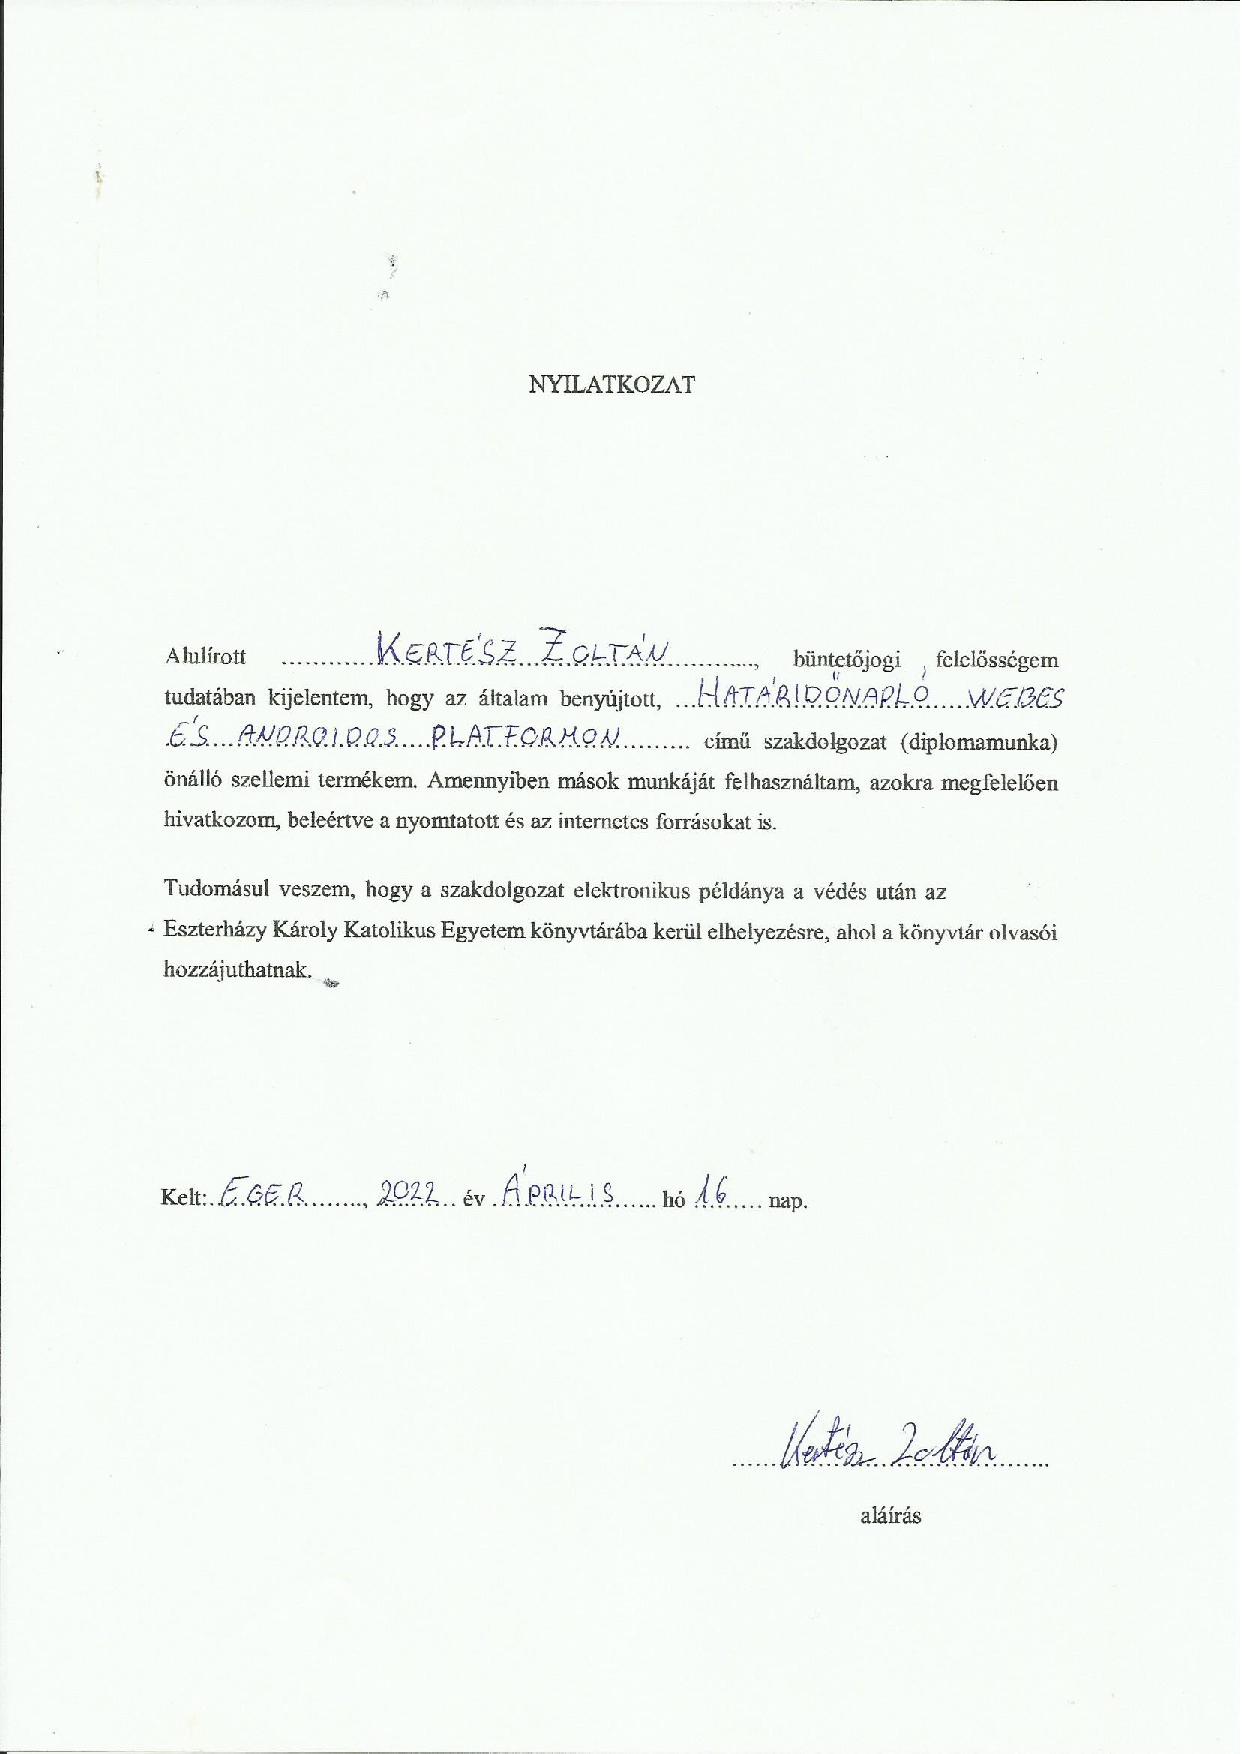
\includepdf[pagecommand={\thispagestyle{empty}}]{nyilatkozat.pdf}
\end{document}